\section{Assessment of Progress}\label{assessment-of-progress}

In this section I will be assessing the progress that I made during the
development of my application.

\subsection{Early Stages}\label{early-stages}

The early stages of my project involved the analysis and design stages
of my application. By performing my competitor analysis I was able set
myself a guideline for what my app should look like and a concept of how
I'd like my users to interact with the app.

I decided that due to developing for Android only I was able to embrace
the material guidelines fully and trying to ensure that my app would
provide a very native Android experience allowing my app to blend in
nicely with the rest of the stock applications on the device included
with the OS.

My app consists of a fairly basic layout, following the guidelines it
was made clear to group functionality by tabs and to only allow actions
associated with the tab; for example if from the lights tab the user
were able to manipulate the lighting, this would go against the design
guidelines.

Some design guidelines posed a few problems and required work to get
them working fully. One such example of this is the coordinator layout
\parencite{coordinator}, to be able to utilise androids latest pop-up
notification system known as the Snackbar, it is required to use a
coordinator layout to wrap the content of the app, by doing this certain
views within the app move and react to the Snackbar being shown.
Although once configured correctly the coordinator layout is easily
added to other views within the application.

\subsection{Development Progress}\label{development-progress}

The development of the application was quite a challenge for many
reasons, many I had not foreseen in the conception or problem analyses
stages of development. As I wanted my app to utilise tabs I had a few
means of achieving this though several involved deprecated methods that
are officially unsupported and are from older versions of Android, these
features would still work as Android still works with these older
methods to ensure older apps are supported.

\subsubsection{Fragments}\label{fragments}

As I would like to develop to the latest standards however I used a
ViewPager with what is known as \cite{fragment}. Fragments are like
Activities in that they hold behaviour and the user interface, a
Fragment however is not a stand-alone aspect of the application and
requires an underlying activity to create and display the Fragment.
Fragments come with many benefits; they can be re-used throughout the
application and multiple fragments can be displayed within a single
activity, this is often seen with communications apps where if viewed in
portrait a list of messages are displayed and when a message is tapped a
new view displays the full message, if both of these views are Fragments
both can be displayed when the device is in landscape, displaying the
list on one side and the entire message on the other.

Fragments however due to being at a higher level running within an
Activity do not have direct access to the application context, with the
application context being the current state of the application such as
the current activity or Fragment being displayed. This posed less of a
challenge and more of a need to learn how to obtain the required context
as in some instances simply using the \lstinline!getContext()! method
worked perfectly, in other instances the need to first get the
application activity and to call the \lstinline!getContext()! method on
that instead caused a few issues when testing my application causing it
to crash if the incorrect one was used.

\subsection{Testing and Feedback}\label{testing-and-feedback}

Testing and feedback have been grouped together as although I was
testing my application during development key testing came from the
users testing my application.

\subsubsection{Debugging}\label{debugging}

The use of the Android Debug Bridge (ADB) \parencite{adb} made
inspecting my application relatively simple as I was able to monitor for
resource usage and any error messages displayed. One issue with the use
of ADB is that it is possible for the device to provide log information
for a lot more than just the application being developed and this could
often cause a lot of information being displayed and obscuring the
information most relevant.

It is possible to filter this information to the application name,
however even the application could often produce large amounts of log
information.

Another issue with the debug information is when an exception error was
thrown or the application crashed there would be a very long stack trace
displaying messages for core OS methods. It is possible however to
produce log information using the provided Log API within Android, this
API can be called using \lstinline!Log.i(tag, message)!, this outputs a
log message with a \emph{tag} string that can be provided. The use of
the tag allows the developer to filter log message by using the tag
allowing for only the messages that developer would like to see be
displayed, greatly reducing the clutter. The \lstinline!Log! API can be
called using different letters as seen in table \ref{table:logkey}.

\begin{longtable}[]{@{}ll@{}}
\caption{Log API Calls \label{table:logkey}}\tabularnewline
\toprule
Letter & Log Type\tabularnewline
\midrule
\endfirsthead
\toprule
Letter & Log Type\tabularnewline
\midrule
\endhead
v & Verbose\tabularnewline
d & Debug\tabularnewline
i & Info\tabularnewline
w & Warning\tabularnewline
e & Error\tabularnewline
\bottomrule
\end{longtable}

Verbose should not be used in a deployed application as much like debug,
the log is stored, however verbose provides more details about the
running application and could present a security risk. `Debug logs are
compiled in but stripped at run-time. Error, warning and info logs are
always kept' \parencite{androidLog}.

\subsection{Problems Encountered}\label{problems-encountered}

Throughout the development of my app many challenges where faced and
problems occurred that required resolution.

\subsubsection{Alarm creation}\label{alarm-creation}

Before developing the alarm aspect of my application I investigated into
how to create alarms within Android, this is were I looked into the
AlarmManager class. The AlarmManager class allows scheduling of an
activity of the application be run at some point in the future.

The AlarmManager allows the specification of the time the alarm should
trigger in either elapsed real-time which is the time from device boot
in milliseconds, or by the Real-Time Clock (RTC) based on the
Coordinated Universal Time Clock (UTC). For my purposes the RTC clock is
the one required as it allows the setting of an alarm to occur at a
specific time instead of occurring a set value of milliseconds in the
future.

Using the AlarmManager it is also possible to set an interval period,
for my application setting the interval to a day would allow the alarm
to be triggered daily at the specified time. Within the developer
guidelines it is recommended to use an inexact repeating alarm as this
allows the device to handle multiple alarms at once when the device
wakes; however I required the alarm to go off at an exact time as
inexact allows for the alarm to be triggered for almost a full interval
of the chosen interval time, in my case a day \parencite{alarmManager}.

\paragraph{Solution}\label{solution}

This is the extent of the AlarmManager class and as such it doesn't
cover any other aspects of what would be regarded as an alarm such as;
an alarm tone, a simple ability to toggle an alarm on/off, hold any
extra details for reoccurring alarms by various days such as
Monday-Friday but not weekends. Due to these limitations I was required
to write my own AlarmManager class that utilised the AlarmManager and
stored the extra functionality that I required.

\subsubsection{Time Picker dialog}\label{time-picker-dialog}

I used the time picker dialog included with Android to allow the users
an attractive way to enter a valid time for the alarm creation.

\begin{figure}
  \centering
    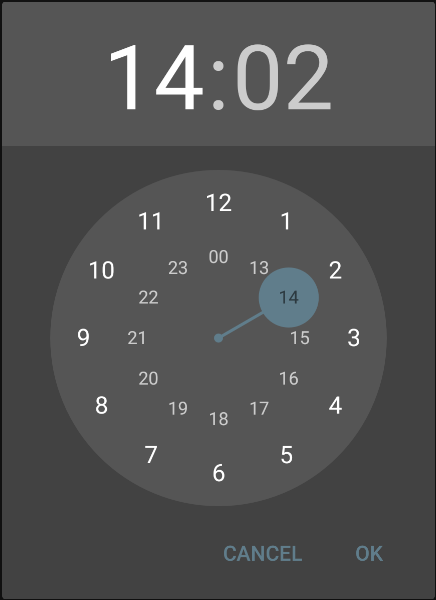
\includegraphics[scale=0.50,keepaspectratio]{Images/components_pickers_time.png}
    \caption{Time Picker Dialog}
\end{figure}

The alarm picker has a method that listens for the confirm activity
within the dialog and from here I am able to call
\lstinline!delayNotification(hourOfDay, minute);! that takes the time
selected within the dialog and create the alarm using my alarm manager.
Due to the time picker dialog method being of a void return time I was
unable to obtain the time chosen from outside of the method, this
restricted how I could utilise the time picker as it required the need
to create the alarm at the same time making adjusting the time of an
existing alarm difficult.

One option for allowing the adjustment of an existing alarm time would
be have global variables for the hour and minute values set within the
time picker listener; I did not like this option however due to the less
predictable nature of my application caused through using global
variables.

An alternative to this approach would be to create a class that would be
able to handle picking the time and be able to return the hour and
minute values. This would be less than ideal as the time picker dialog
would be created in a different class than the alarm fragment but
requires the need to be able to displayed on the UI thread and this
posed certain problems.

\paragraph{Solution}\label{solution-1}

I feel there is still a better way to handle the time picker, due to
working on other aspects of my application however I ran out of time to
be able to implement a better method for selecting the time for the
alarm. The user is able to pick their alarm time as required though by
having the alarm creation called from within the dialog listener there
is no way to edit an existing alarm, this means the user would need to
create a new alarm and delete the old one if they would like to set an
alarm for a different time.

\subsubsection{Handling Pending intents}\label{handling-pending-intents}

Within Android there is a need to specify an Intent to start a new
activity or fragment. The Intent is a fairly simple class that allows
for activities to be called/started and provides a data structure that
holds the activities and tasks in a back stack, this allows for the use
of the back button by closing the current activity/task the app can pop
the activity from the back stack and present the previous element in the
stack.

A new intent is created as follows:

\begin{lstlisting}
Intent intentName = new Intent(activity.class, context)

startIntentForResult(intentName, result)
\end{lstlisting}

It is also simple to pass data between intents by the use of
\lstinline!addExtra! which provides a means to add a key-value pair that
can be accessed. The use of the result in the above Intent example will
request that the intent return a response, this can be used to handle
various exit values of the intent to be able handle errors or developer
specified return values.

The use of a Pending Intent allows for a foreign application to launch
an Intent with the permissions of the application the Pending Intent was
specified from. This is useful as it allows for an Intent to be launched
by the NotificationManager and the AlarmManager, allowing for an
activity to be launched even when the application is not open.

Cancelling pending intents is not as simple as creating one, cancelling
a pending intent requires for a new pending intent to be specified just
as the original was and to pass \lstinline!.cancel()! as the last
method, if the pending intent exists it will be cancelled and if it did
not nothing else will happen.

\paragraph{Solution}\label{solution-2}

By storing a reference to any created pending intents, it becomes
trivial to be able to cancel a pending intent, by simply obtaining a
stored reference and calling \lstinline!.cancel()!.

\subsubsection{Storing Objects}\label{storing-objects}

For my alarms to be persistent I was required to store the alarm objects
by some means so that they could be created, updated or deleted.

Within Android there are several methods for storing data persistently
these include using; Shared Preferences, internal/external storage or an
SQL database. Each of these storage solutions come with their benefits
and restrictions.

\paragraph{Shared Preferences}\label{shared-preferences}

Shared Preferences allows the storage of key-value pairs within storage,
by storing the key-value pair data can be stored and accessed by the
usage of the key. Shared preferences although simple to use has the
restriction of only being able to store string values within the value
of the key, as such this greatly restricts what can be stored.

It is possible to store an object within the shared preferences by
converting the data into a JSON object by use of an interface library.
This is mostly suited towards small and simple objects as changing a
stored value would involve retrieving the entire object from memory,
altering the JSON associated with the change and then storing the data
back as a JSON object.

Due to these limitations it would be a poor choice for storing my Alarm
objects.

\paragraph{Internal/External storage}\label{internalexternal-storage}

Storing data to the internal and external storage is about as
challenging as storing data within the shared preferences. All data
stored in the internal storage can only be accessed by the application,
preventing other applications or direct user access to retrieve the
data. External storage allows for the data to be accessed freely by
other applications or directly by the user by browsing through the
device file system.

Both forms of storage however are better suited for media and files such
as images, music or text files. Again it would be possible to store the
object as a JSON object and access it much like how shared preferences
would provide access and due to this comes with similar restrictions.

\paragraph{Database}\label{database}

By using a database this is the most involved method for storing object
data with each row of the database table able to store an object
variable and provide direct access to each variable through interfacing
with the database.

The database can be interacted with directly by executing raw SQL
statements and queries or by the use of a database helper which allows a
method means of interacting with the database.

A database is stored with the internal storage and as such only allows
access to the application and prevents access from external use, this is
ideal as there is no need for another application or for the user to
have direct access to the database.

\subsubsection{Alarm Solution}\label{alarm-solution}

I used an SQLite database as it provides all the functionality I
required and kept my project simple. One restriction of using SQLite is
that there is no dedicated Boolean type and instead a Boolean value can
be stored as an integer value with 0 representing \emph{false} and 1
representing \emph{true}, this was a simple enough restriction to work
around.

Within a day I was able to get my alarms stored persistently and another
day to be able to completely implement all required Create, read, update
and delete (CRUD) operations.

\subsection{Lessons Learned}\label{lessons-learned}

Knowing target market is important due to the variance of deprecated
methods and functions. It is possible to develop for only the latest
version of Android and this comes with the benefits of being able to use
the latest version of Java, as of writing this the latest is version 8;
this version comes with many useful features from the use of lambda
functions, to the ability to use mapping functions and allow for the
simple parallelisation over a group of elements, of which can lead to
improvements in both speed of the action called and in the way the
function is called by the developer leading to more readable code and a
better ability to reason about what is happening.

However due to the current market share of the latest version of Android
and the relatively slow adoption rate of newer version by phone
manufacturers when newer versions are released, a majority of the market
would not be catered for, thus limiting the reach of the application.

The separation between UI and the rest of the application can cause
certain issues; for example running code from within a fragment that is
not the current running activity will cause a
\lstinline!runOnUiThread undefined! error in most cases, this is because
a fragment does not have a \lstinline!runOnUiThread! method as it runs
as the fragment may have become detached from the activity and so the
fragment may have been destroyed by the time the method comes to run.
Due to the unknown nature of the fragment it is required to get the
current activity when running and to check that the activity is not null
before running.

Application security is good in Android, through the use of sand-boxing
and defaulting to keeping data private, requiring the developer to
specify actions that are \emph{unsafe} it is possible to prevent app
hijacking or having data leaked from within the app. Devices running the
latest versions of Android are encrypted by default, this provides an
extra level of protection on a device as when the device is off it is
harder to retrieve data from the device where it used to be an attack
vector by exploiting the ADB to gain access to the internal storage.

This extra level of security is not of much importance to my
application, it is something learned through the investigation of the
different means of storing data on the device however and could be
useful for future developments.
